\chapter{RESULTADOS}
\label{ch:resultados}

En el presente capítulo, se muestra el análisis de los resultados obtenidos a partir de la simulación e implementación de las estrategias de control desarrolladas en el marco metodológico. Se presentan las conexiones del nodo sensor, los resultados de simulación del controlador PI/PID, los resultados experimentales del controlador PI/PID y la validación de la página web para la lectura de los sensores.

\section{Conexiones del nodo sensor}

Se realizaron las conexiones entre la placa de prototipado Arduino UNO, el sensor MH-Z19B y el módulo LoRa E220-900T30D como se muestra en la figura \ref{fig:diagrama_conexiones}. Los pines utilizados para cada componente se detallan en la tabla \ref{tabla:conexiones}.




\begin{figure}[H]
    \centering
    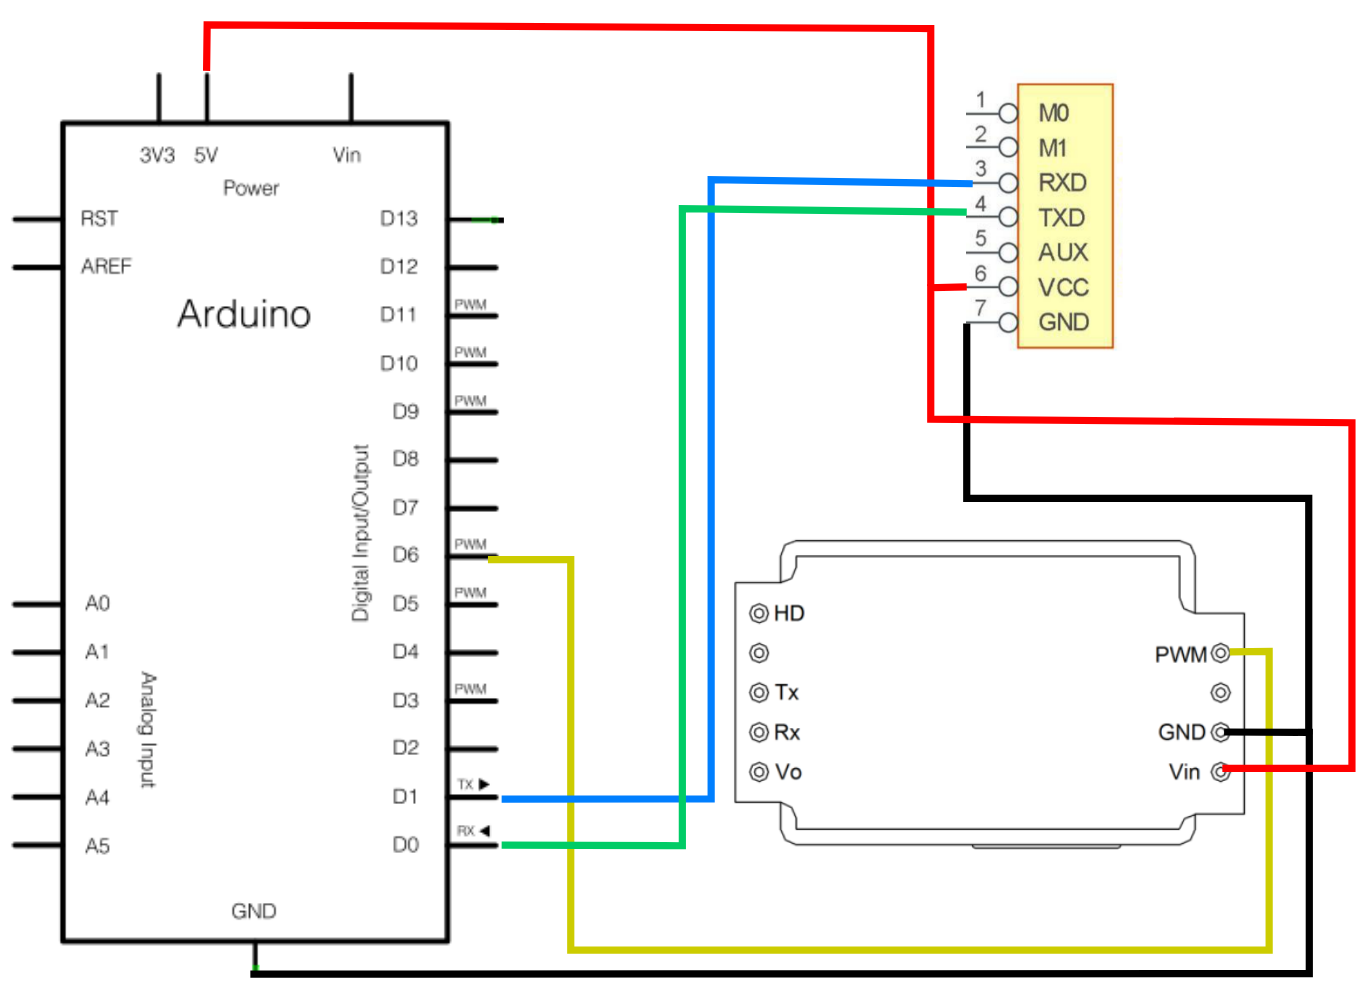
\includegraphics[width=\linewidth]{images/capitulo4/diagrama_conexiones.png}
    \caption{Diagrama de conexiones del nodo sensor}
    \label{fig:diagrama_conexiones}
\end{figure}



\begin{table}[h!]
    \centering
    \renewcommand{\arraystretch}{1.5}
    \caption{Conexiones para el nodo sensor}
    \label{tabla:conexiones}
    \begin{tabular}{|c|c|c|}
        \hline
        \textbf{Pines del Arduino UNO} & \textbf{Pines del MH-Z19B} & \textbf{Pines del E220-900T30D} \\ \hline
        GND                            & GND                        & GND                             \\ \hline
        5V                             & VCC                        & VCC                             \\ \hline
        D6                             & PWM                        & -                               \\ \hline
        RX (D0)                        & -                          & TX                              \\ \hline
        TX (D1)                        & -                          & RX                              \\ \hline
    \end{tabular}
\end{table}



\section{Resultados de simulación de los controladores}

\subsection{Resultados de simulación del controlador PI/PID}

En esta sección se presentan los resultados obtenidos mediante la simulación del controlador PI/PID aplicado al modelo de concentración de CO\(_2\) en el aula. La simulación considera una condición inicial elevada de CO\(_2\), un valor de referencia de 900 ppm y la actuación de cinco ventiladores como mecanismo de mitigación activa. Los resultados permiten analizar la evolución de la concentración de CO\(_2\), el esfuerzo de control aplicado y el caudal efectivo generado por el sistema de ventilación.

\begin{figure}[H]
    \centering
    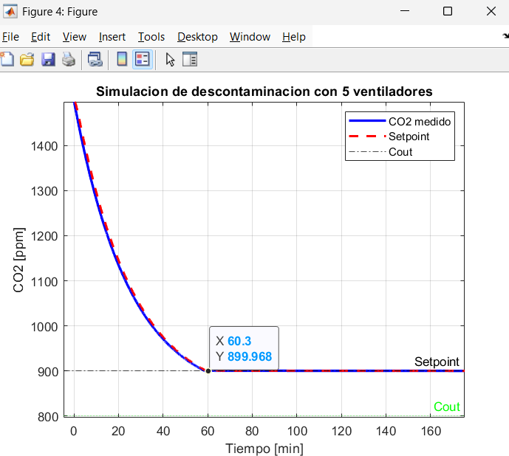
\includegraphics[width=0.9\linewidth]{images/capitulo4/PI_CO2_Simulacion.png}
    \caption{Respuesta simulada de la concentración de CO\(_2\) con controlador PI/PID.}
    \label{fig:PI_CO2_Simulacion}
\end{figure}

Como se observa en la Figura \ref{fig:PI_CO2_Simulacion}, la concentración de CO\(_2\) inicia en un valor cercano a 1500 ppm y disminuye progresivamente como consecuencia de la ventilación aplicada por el controlador. El sistema alcanza el valor de referencia de 900 ppm aproximadamente a los 60.3 minutos, con una concentración de 899.968 ppm. A partir de ese instante, la respuesta se mantiene próxima al setpoint, lo que evidencia que el controlador PI/PID permite reducir la concentración de CO\(_2\) desde una condición inicial desfavorable hasta el nivel objetivo establecido.

\begin{figure}[H]
    \centering
    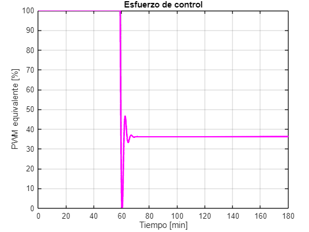
\includegraphics[width=0.9\linewidth]{images/capitulo4/PI_Esfuerzo_Simulacion.png}
    \caption{Esfuerzo de control simulado del controlador PI/PID.}
    \label{fig:PI_Esfuerzo_Simulacion}
\end{figure}

La Figura \ref{fig:PI_Esfuerzo_Simulacion} muestra el esfuerzo de control equivalente en porcentaje de PWM. Durante los primeros 60 minutos, la señal de control se mantiene cercana al 100\%, debido a que la concentración de CO\(_2\) se encuentra muy por encima del valor de referencia. Cuando el sistema alcanza la zona del setpoint, el esfuerzo de control disminuye de manera brusca y presenta una breve oscilación transitoria. Posteriormente, la señal se estabiliza alrededor de un valor aproximado de 35\% a 36\%, suficiente para mantener la concentración de CO\(_2\) cercana al valor objetivo.

\begin{figure}[H]
    \centering
    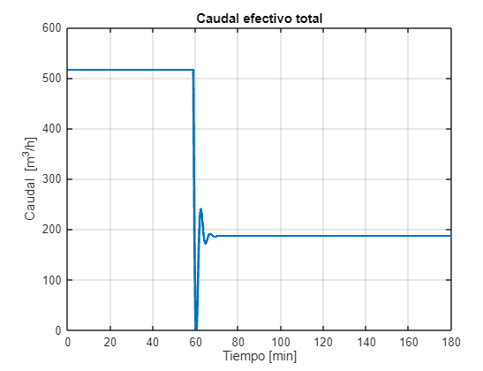
\includegraphics[width=0.9\linewidth]{images/capitulo4/PI_Caudal_Simulacion.png}
    \caption{Caudal efectivo simulado generado por el sistema de ventilación con controlador PI/PID.}
    \label{fig:PI_Caudal_Simulacion}
\end{figure}

En la Figura \ref{fig:PI_Caudal_Simulacion} se presenta el caudal efectivo total generado por el sistema de ventilación. Durante la etapa inicial, el caudal se mantiene aproximadamente en 515 m\(^3\)/h, correspondiente a una actuación máxima de los ventiladores. Alrededor de los 60 minutos, cuando la concentración de CO\(_2\) alcanza el setpoint, el caudal disminuye rápidamente y presenta un comportamiento transitorio asociado al reajuste del controlador. Finalmente, el caudal se estabiliza cerca de 185 a 190 m\(^3\)/h, lo que indica que el sistema reduce la ventilación una vez alcanzada la concentración objetivo, pero mantiene un caudal mínimo necesario para conservar el equilibrio del ambiente.

En conjunto, los resultados de simulación del controlador PI/PID muestran una respuesta estable y progresiva para la reducción de CO\(_2\). El tiempo aproximado de llegada al setpoint fue de 60.3 minutos, con una actuación máxima durante la etapa inicial y una reducción posterior del esfuerzo de control hasta un valor estacionario cercano al 35\%. Este comportamiento demuestra que el controlador PI/PID es capaz de disminuir la concentración de CO\(_2\) y ajustar la ventilación de manera progresiva, por lo que estos resultados sirven como referencia para comparar posteriormente el desempeño de las estrategias Fuzzy PI, Fuzzy PI agresiva y LQR.


\subsection{Resultados de simulación del controlador Fuzzy PI base}

En esta sección se presentan los resultados obtenidos mediante la simulación del controlador Fuzzy PI base aplicado al modelo de concentración de CO\(_2\) del aula. A diferencia del controlador PI/PID, esta estrategia emplea una base de reglas difusas para determinar el porcentaje de ventilación en función del error de concentración de CO\(_2\) y la acumulación del error. La simulación permite analizar la evolución de la concentración de CO\(_2\), el error de control, el esfuerzo de control aplicado y el caudal efectivo generado por los ventiladores.

\begin{figure}[H]
    \centering
    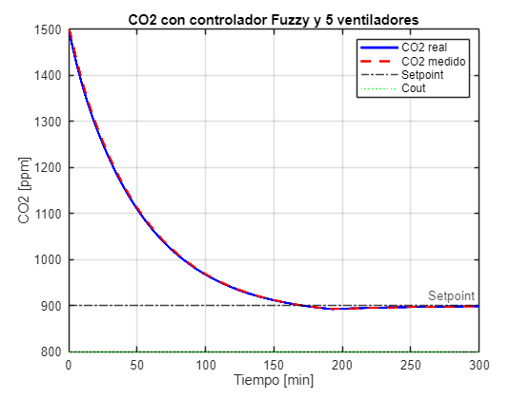
\includegraphics[width=0.9\linewidth]{images/capitulo4/FUZZY_CO2_Simulacion.png}
    \caption{Respuesta simulada de la concentración de CO\(_2\) con controlador Fuzzy PI base.}
    \label{fig:fuzzy_co2_simulacion}
\end{figure}

Como se observa en la Figura \ref{fig:fuzzy_co2_simulacion}, la concentración de CO\(_2\) inicia en un valor cercano a 1500 ppm y disminuye progresivamente debido a la acción del controlador Fuzzy PI. La respuesta presenta una reducción suave y continua, alcanzando una zona cercana al setpoint de 900 ppm aproximadamente entre los 170 y 180 minutos. Posteriormente, la concentración desciende ligeramente por debajo del valor de referencia, llegando a una zona aproximada de 890 ppm alrededor de los 190 a 210 minutos, para luego estabilizarse nuevamente cerca del setpoint. Este comportamiento muestra que el controlador Fuzzy PI logra reducir la concentración de CO\(_2\), aunque con una respuesta más lenta que la obtenida con el controlador PI/PID simulado.

\begin{figure}[H]
    \centering
    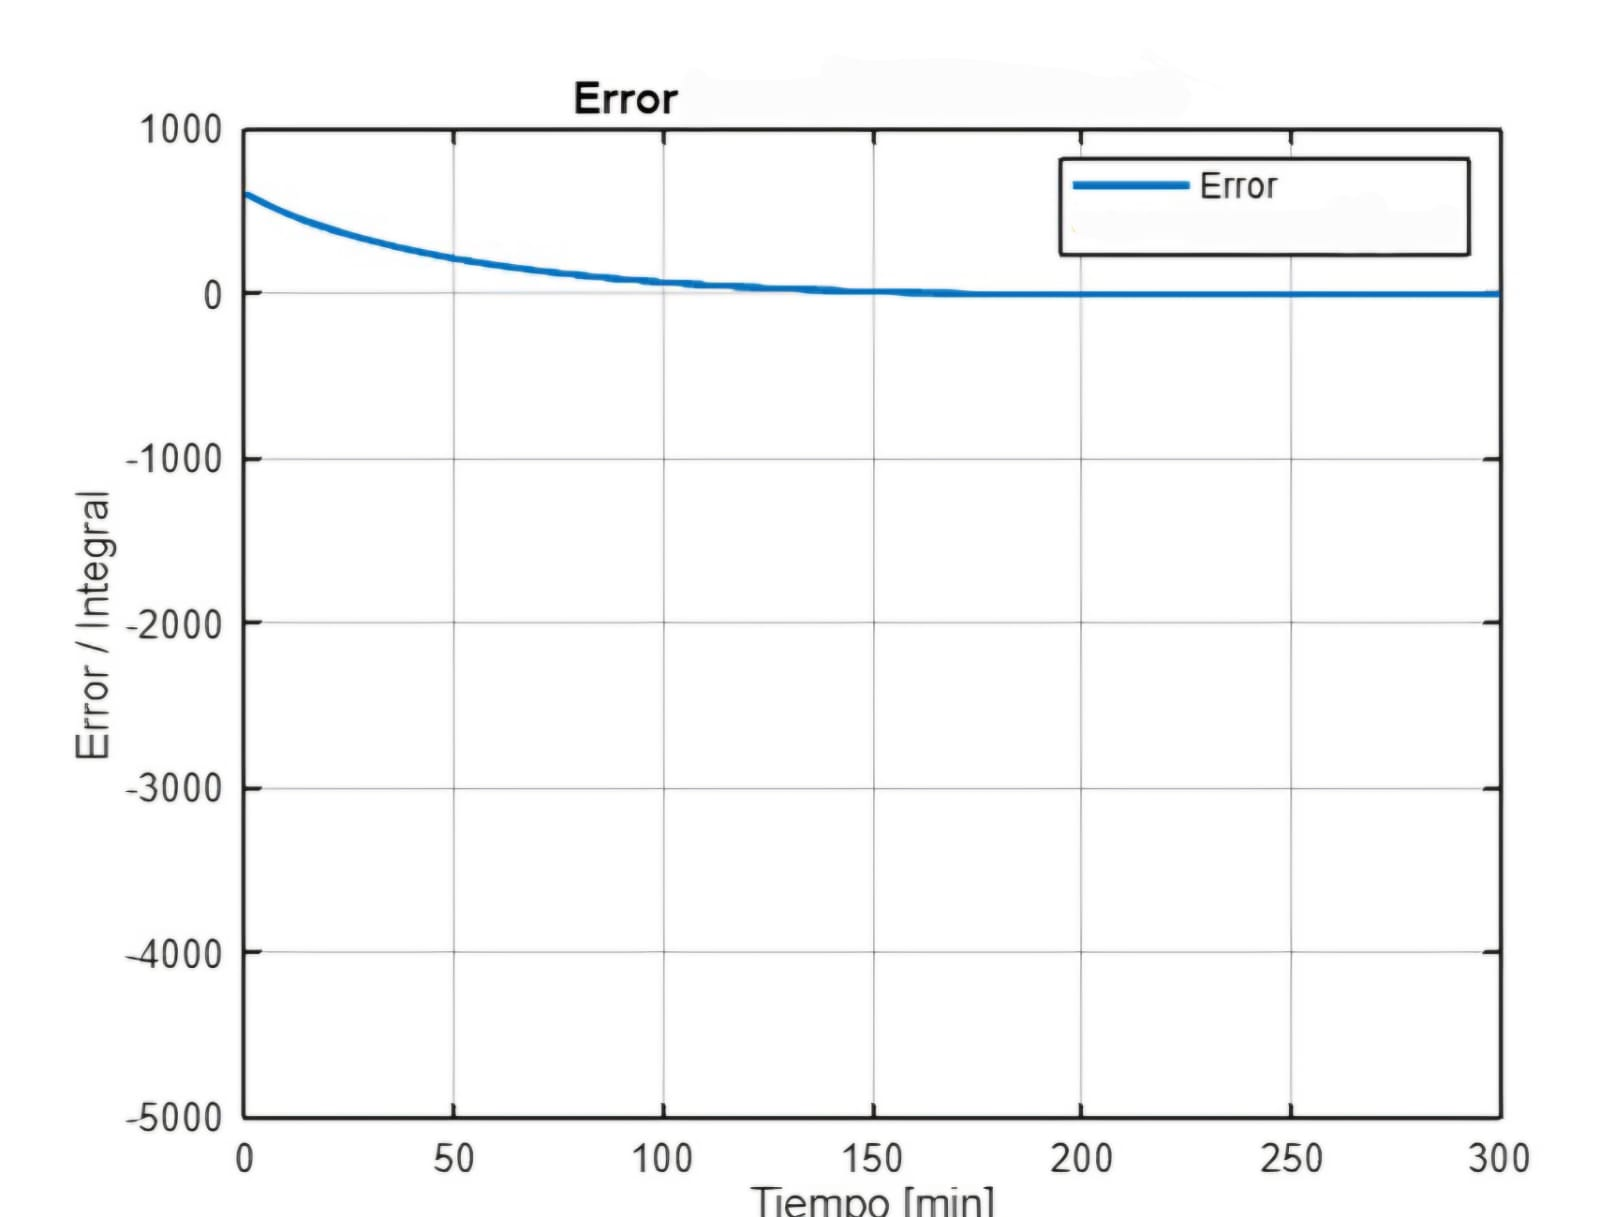
\includegraphics[width=0.9\linewidth]{images/capitulo4/FUZZY_Error_Simulacion.jpg}
    \caption{Evolución del error de control durante la simulación del controlador Fuzzy PI base.}
    \label{fig:fuzzy_error_simulacion}
\end{figure}

La Figura \ref{fig:fuzzy_error_simulacion} muestra la evolución del error de control durante la simulación. Al inicio, el error es elevado, con un valor aproximado de 600 ppm, debido a que la concentración de CO\(_2\) se encuentra muy por encima del setpoint. A medida que avanza la ventilación, el error disminuye de forma gradual hasta aproximarse a cero alrededor de los 150 a 180 minutos. Luego, el error se vuelve ligeramente negativo durante un intervalo corto, lo cual coincide con la reducción de la concentración de CO\(_2\) por debajo del setpoint. Finalmente, el error tiende nuevamente a cero, evidenciando una estabilización progresiva del sistema.

\begin{figure}[H]
    \centering
    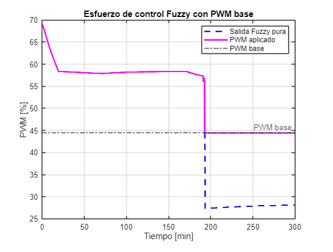
\includegraphics[width=0.9\linewidth]{images/capitulo4/FUZZY_Esfuerzo_Simulacion.png}
    \caption{Esfuerzo de control simulado del controlador Fuzzy PI base.}
    \label{fig:fuzzy_esfuerzo_simulacion}
\end{figure}

En la Figura \ref{fig:fuzzy_esfuerzo_simulacion} se observa el esfuerzo de control generado por el controlador Fuzzy PI. La salida Fuzzy pura inicia cerca del 69\% de PWM y disminuye rápidamente hasta una zona aproximada de 58\% durante los primeros minutos. Posteriormente, la acción de control se mantiene casi constante entre 57\% y 59\% hasta cerca de los 180 minutos, lo cual indica una actuación moderada y sostenida de los ventiladores. Cuando el sistema se aproxima al setpoint, la salida Fuzzy pura disminuye bruscamente hasta valores cercanos al 27\% o 28\%. Sin embargo, debido a la incorporación de un PWM base, el PWM aplicado se mantiene alrededor de 44\% a 45\%, evitando que la ventilación caiga por debajo del caudal mínimo requerido para sostener la concentración de CO\(_2\) cercana al valor de referencia.

\begin{figure}[H]
    \centering
    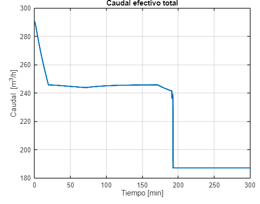
\includegraphics[width=0.9\linewidth]{images/capitulo4/FUZZY_Caudal_Simulacion.png}
    \caption{Caudal efectivo simulado generado por el sistema de ventilación con controlador Fuzzy PI base.}
    \label{fig:fuzzy_caudal_simulacion}
\end{figure}

La Figura \ref{fig:fuzzy_caudal_simulacion} presenta el caudal efectivo total generado por el sistema de ventilación. Al inicio de la simulación, el caudal se encuentra cerca de 290 m\(^3\)/h y disminuye rápidamente hasta aproximadamente 245 m\(^3\)/h durante los primeros minutos. Luego, el caudal se mantiene prácticamente estable entre 242 y 245 m\(^3\)/h hasta cerca de los 180 minutos. Al aproximarse la concentración de CO\(_2\) al setpoint, el caudal disminuye de forma abrupta hasta un valor cercano a 187 m\(^3\)/h, manteniéndose estable durante la etapa final de la simulación. Este comportamiento es coherente con la reducción del esfuerzo de control observada en la Figura \ref{fig:fuzzy_esfuerzo_simulacion}.

En conjunto, los resultados de simulación del controlador Fuzzy PI base muestran una respuesta estable, suave y progresiva para la reducción de CO\(_2\). El sistema logra aproximarse al setpoint de 900 ppm en un tiempo estimado de 170 a 180 minutos, con un esfuerzo de control moderado y sostenido durante la mayor parte de la simulación. En comparación con el controlador PI/PID simulado, el Fuzzy PI base presenta una respuesta más lenta, pero utiliza un menor esfuerzo inicial de ventilación, ya que no requiere mantener el PWM en 100\% durante la etapa inicial. Esto lo convierte en una estrategia menos agresiva, pero más gradual en términos de actuación sobre los ventiladores.


\subsection{Resultados de simulación del controlador Fuzzy PI agresivo}

En esta sección se presentan los resultados obtenidos mediante la simulación del controlador Fuzzy PI agresivo. Esta variante fue diseñada con el propósito de incrementar la acción de ventilación ante errores medios y altos de concentración de CO\(_2\), utilizando una base de reglas más intensa y una salida difusa orientada a mayores valores de PWM. De esta manera, se busca reducir el tiempo de llegada a la zona cercana al setpoint, aunque con un mayor esfuerzo de control respecto al Fuzzy PI base.

\begin{figure}[H]
    \centering
    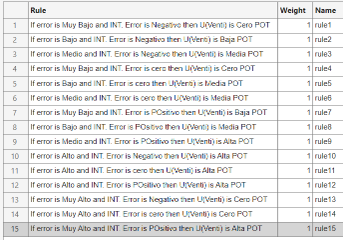
\includegraphics[width=0.9\linewidth]{images/capitulo4/Fuzzy_Agresivo_Reglas_Simulacion.png}
    \caption{Base de reglas utilizada en la simulación del controlador Fuzzy PI agresivo.}
    \label{fig:fuzzy_agresivo_reglas_simulacion}
\end{figure}

La Figura \ref{fig:fuzzy_agresivo_reglas_simulacion} muestra la base de reglas utilizada para la variante agresiva del controlador Fuzzy PI. En esta configuración, las combinaciones asociadas a errores medios, altos y muy altos generan con mayor frecuencia salidas de potencia media o alta. Esto permite que el sistema incremente la ventilación en etapas tempranas de la simulación, especialmente cuando la concentración de CO\(_2\) se encuentra considerablemente por encima del valor de referencia.

\begin{figure}[H]
    \centering
    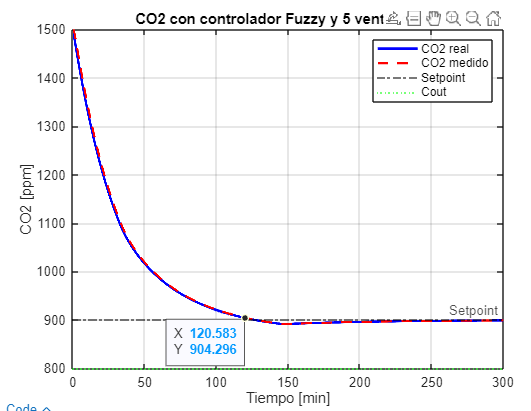
\includegraphics[width=0.9\linewidth]{images/capitulo4/Fuzzy_Agresivo_CO2_Simulacion.png}
    \caption{Respuesta simulada de la concentración de CO\(_2\) con controlador Fuzzy PI agresivo.}
    \label{fig:fuzzy_agresivo_co2_simulacion}
\end{figure}

Como se observa en la Figura \ref{fig:fuzzy_agresivo_co2_simulacion}, la concentración de CO\(_2\) inicia en un valor cercano a 1500 ppm y disminuye de forma sostenida debido a la acción del controlador. La respuesta ingresa a una zona cercana al setpoint alrededor de los 120.6 minutos, donde la concentración medida es aproximadamente 904.296 ppm. Posteriormente, el sistema continúa reduciendo ligeramente la concentración hasta ubicarse por debajo del valor de referencia, para luego estabilizarse gradualmente en torno a 900 ppm. En comparación con el Fuzzy PI base, esta variante alcanza la zona cercana al setpoint en menor tiempo, evidenciando una respuesta más rápida.

\begin{figure}[H]
    \centering
    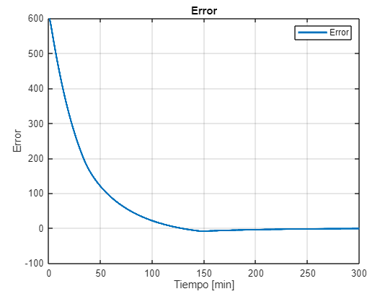
\includegraphics[width=0.9\linewidth]{images/capitulo4/Fuzzy_Agresivo_Error_Simulacion.png}
    \caption{Evolución del error de control durante la simulación del controlador Fuzzy PI agresivo.}
    \label{fig:fuzzy_agresivo_error_simulacion}
\end{figure}

La Figura \ref{fig:fuzzy_agresivo_error_simulacion} presenta la evolución del error de control. Al inicio de la simulación, el error es aproximadamente de 600 ppm, debido a que la concentración inicial de CO\(_2\) se encuentra muy por encima del setpoint. Durante los primeros minutos, el error disminuye rápidamente como consecuencia del mayor esfuerzo de ventilación aplicado por el controlador agresivo. Cerca de los 120 a 150 minutos, el error se aproxima a cero y posteriormente toma valores ligeramente negativos, lo que indica que la concentración de CO\(_2\) desciende temporalmente por debajo del valor de referencia. Finalmente, el error tiende nuevamente a cero, mostrando la estabilización progresiva del sistema.

\begin{figure}[H]
    \centering
    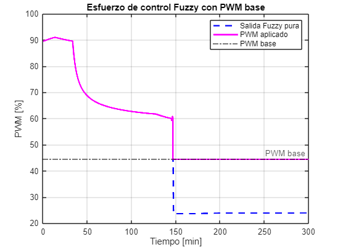
\includegraphics[width=0.9\linewidth]{images/capitulo4/Fuzzy_Agresivo_Esfuerzo_Simulacion.png}
    \caption{Esfuerzo de control simulado del controlador Fuzzy PI agresivo.}
    \label{fig:fuzzy_agresivo_esfuerzo_simulacion}
\end{figure}

En la Figura \ref{fig:fuzzy_agresivo_esfuerzo_simulacion} se muestra el esfuerzo de control generado por el controlador Fuzzy PI agresivo. Durante la etapa inicial, el PWM aplicado se mantiene cercano al 90\%, lo que refleja una acción de ventilación más intensa que la observada en el Fuzzy PI base. Luego, la señal disminuye progresivamente hasta valores cercanos al 60\% alrededor de los 140 minutos. Cuando el sistema alcanza la zona del setpoint, la salida Fuzzy pura cae hasta aproximadamente 24\% a 25\%; sin embargo, debido al PWM base, el PWM aplicado se mantiene alrededor de 44\% a 45\%. Este comportamiento permite conservar una ventilación mínima para sostener la concentración de CO\(_2\) cerca del valor objetivo.

\begin{figure}[H]
    \centering
    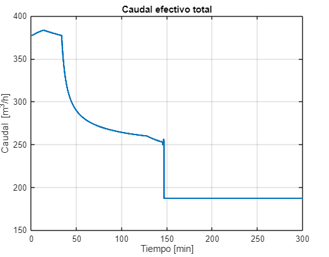
\includegraphics[width=0.9\linewidth]{images/capitulo4/Fuzzy_Agresivo_Caudal_Simulacion.png}
    \caption{Caudal efectivo simulado generado por el sistema de ventilación con controlador Fuzzy PI agresivo.}
    \label{fig:fuzzy_agresivo_caudal_simulacion}
\end{figure}

La Figura \ref{fig:fuzzy_agresivo_caudal_simulacion} muestra el caudal efectivo total producido por los ventiladores durante la simulación. Al inicio, el caudal se encuentra aproximadamente entre 375 y 380 m\(^3\)/h, valor superior al observado en el Fuzzy PI base. Posteriormente, el caudal disminuye de manera progresiva conforme la concentración de CO\(_2\) se aproxima al setpoint, ubicándose cerca de 260 m\(^3\)/h alrededor de los 120 a 140 minutos. Finalmente, cuando la respuesta entra en la zona cercana al valor de referencia, el caudal desciende abruptamente hasta aproximadamente 188 m\(^3\)/h, manteniéndose estable durante la etapa final de la simulación. Esta evolución es coherente con la disminución del esfuerzo de control mostrada previamente.

En conjunto, los resultados de simulación del controlador Fuzzy PI agresivo muestran una respuesta más rápida que la obtenida con el Fuzzy PI base. La concentración de CO\(_2\) ingresa a una zona cercana al setpoint aproximadamente a los 120.6 minutos, frente al comportamiento más lento del Fuzzy PI base. No obstante, esta mejora en rapidez se obtiene a costa de un mayor esfuerzo inicial de control, ya que el PWM aplicado inicia cerca del 90\% y el caudal efectivo alcanza valores próximos a 380 m\(^3\)/h. Por ello, esta variante puede considerarse más adecuada cuando se prioriza una reducción más rápida de CO\(_2\), aunque implica una mayor demanda de ventilación durante la etapa inicial.


\subsection{Resultados de simulación del controlador LQR}

En esta sección se presentan los resultados obtenidos mediante la simulación del controlador LQR aplicado al modelo de concentración de CO\(_2\) del aula. Esta estrategia de control se basa en la realimentación de estados y busca regular la ventilación considerando un compromiso entre la rapidez de respuesta y el esfuerzo de control aplicado. Para la simulación se mantuvieron las mismas condiciones generales empleadas en las estrategias anteriores, considerando una concentración inicial elevada de CO\(_2\), un setpoint de 900 ppm y la actuación de cinco ventiladores.

\begin{figure}[H]
    \centering
    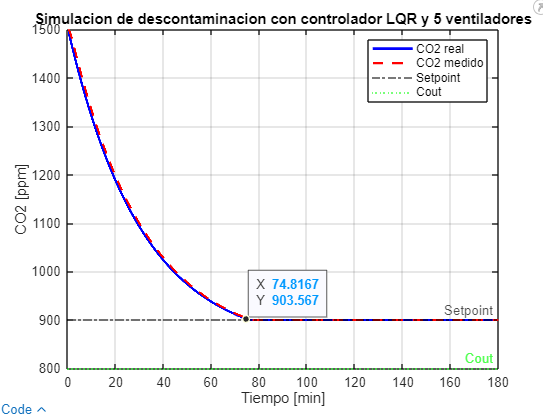
\includegraphics[width=0.9\linewidth]{images/capitulo4/LQR_CO2_Simulacion.png}
    \caption{Respuesta simulada de la concentración de CO\(_2\) con controlador LQR.}
    \label{fig:lqr_co2_simulacion}
\end{figure}

Como se observa en la Figura \ref{fig:lqr_co2_simulacion}, la concentración de CO\(_2\) inicia en un valor cercano a 1500 ppm y disminuye progresivamente debido a la acción del controlador LQR. La respuesta alcanza una zona cercana al setpoint alrededor de los 74.8 minutos, donde la concentración medida es aproximadamente 903.567 ppm. Posteriormente, el sistema continúa acercándose al valor de referencia de 900 ppm sin presentar oscilaciones importantes. Este comportamiento evidencia que el controlador LQR permite reducir la concentración de CO\(_2\) de manera estable y con un tiempo de respuesta menor al observado en los controladores Fuzzy PI base y Fuzzy PI agresivo.

\begin{figure}[H]
    \centering
    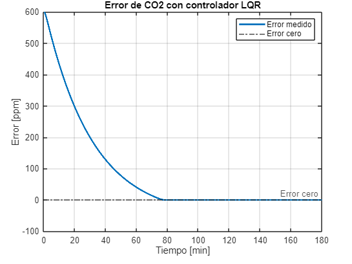
\includegraphics[width=0.9\linewidth]{images/capitulo4/LQR_Error_Simulacion.png}
    \caption{Evolución del error de control durante la simulación del controlador LQR.}
    \label{fig:lqr_error_simulacion}
\end{figure}

La Figura \ref{fig:lqr_error_simulacion} muestra la evolución del error de CO\(_2\) durante la simulación. Al inicio, el error es aproximadamente de 600 ppm, debido a la diferencia entre la concentración inicial de 1500 ppm y el setpoint de 900 ppm. Conforme actúa el sistema de ventilación, el error disminuye de forma continua hasta aproximarse a cero alrededor de los 75 minutos. A diferencia de otras respuestas, no se observa un sobrepaso negativo considerable, lo cual indica que el sistema se aproxima al valor de referencia de manera controlada y estable.

\begin{figure}[H]
    \centering
    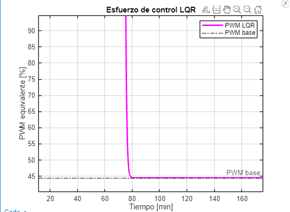
\includegraphics[width=0.9\linewidth]{images/capitulo4/LQR_Esfuerzo_Simulacion.png}
    \caption{Esfuerzo de control simulado del controlador LQR.}
    \label{fig:lqr_esfuerzo_simulacion}
\end{figure}

En la Figura \ref{fig:lqr_esfuerzo_simulacion} se presenta el esfuerzo de control generado por el controlador LQR, expresado como PWM equivalente. Durante la etapa inicial de la simulación, el PWM aplicado se mantiene en un valor elevado, cercano al 90\%, debido a que la concentración de CO\(_2\) se encuentra muy por encima del setpoint. Alrededor de los 75 minutos, cuando el sistema se aproxima al valor de referencia, el esfuerzo de control disminuye rápidamente hasta ubicarse cerca del PWM base, aproximadamente entre 44\% y 45\%. Esto indica que el controlador reduce la ventilación una vez alcanzada la zona objetivo, manteniendo solo la acción necesaria para sostener la concentración cercana al setpoint.

\begin{figure}[H]
    \centering
    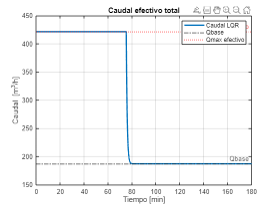
\includegraphics[width=0.9\linewidth]{images/capitulo4/LQR_Caudal_Simulacion.png}
    \caption{Caudal efectivo simulado generado por el sistema de ventilación con controlador LQR.}
    \label{fig:lqr_caudal_simulacion}
\end{figure}

La Figura \ref{fig:lqr_caudal_simulacion} muestra el caudal efectivo total generado por los ventiladores durante la simulación. En la etapa inicial, el caudal se mantiene aproximadamente en 420 m\(^3\)/h, correspondiente a una alta demanda de ventilación para reducir rápidamente la concentración de CO\(_2\). Cuando el sistema se aproxima al setpoint, cerca de los 75 minutos, el caudal disminuye de manera abrupta hasta un valor cercano a 188 m\(^3\)/h. Este valor se mantiene prácticamente constante durante la etapa final, lo cual es coherente con la reducción del esfuerzo de control observada en la Figura \ref{fig:lqr_esfuerzo_simulacion}.

En conjunto, los resultados de simulación del controlador LQR muestran una respuesta estable y rápida frente a una concentración inicial elevada de CO\(_2\). El sistema alcanza una zona cercana al setpoint aproximadamente a los 74.8 minutos, con una concentración de 903.567 ppm, y luego se estabiliza alrededor del valor de referencia sin oscilaciones significativas. En comparación con los controladores Fuzzy PI base y Fuzzy PI agresivo, el LQR presenta un menor tiempo de llegada a la zona objetivo. Sin embargo, esta mejora se obtiene mediante un esfuerzo inicial elevado, con un PWM cercano al 90\% y un caudal aproximado de 420 m\(^3\)/h durante la etapa inicial. Por ello, el controlador LQR representa una estrategia eficiente para reducir el tiempo de mitigación, manteniendo una respuesta estable después de alcanzar el setpoint.


\subsection{Comparación general de los controladores simulados}

Con el propósito de evaluar el desempeño de las estrategias de control implementadas en simulación, se realizó una comparación entre el controlador PI/PID, el controlador Fuzzy PI base, el controlador Fuzzy PI agresivo y el controlador LQR. Para esta comparación se consideraron criterios como el tiempo aproximado de llegada a la zona cercana al setpoint, el esfuerzo inicial de control, el caudal efectivo inicial, la estabilidad de la respuesta y la observación general del comportamiento de cada estrategia.

\begin{table}[H]
    \centering
    \renewcommand{\arraystretch}{1.4}
    \caption{Comparación de desempeño de los controladores simulados}
    \label{tabla:comparacion_controladores_simulados}
    \resizebox{\textwidth}{!}{
    \begin{tabular}{|p{3cm}|p{3cm}|p{3cm}|p{3cm}|p{4.5cm}|}
        \hline
        \textbf{Controlador} & \textbf{Tiempo aprox. de llegada al setpoint} & \textbf{Esfuerzo inicial de control} & \textbf{Caudal inicial aprox.} & \textbf{Observación general} \\ \hline

        PI/PID & 60.3 min & 100\% PWM & 515 m\(^3\)/h & Presenta la respuesta más rápida en simulación, pero requiere la actuación máxima de los ventiladores durante la etapa inicial. \\ \hline

        Fuzzy PI base & 170--180 min & 69\% PWM aprox. & 290 m\(^3\)/h & Presenta una respuesta más lenta, pero con una acción de control más suave y menor demanda inicial de ventilación. \\ \hline

        Fuzzy PI agresivo & 120.6 min & 90\% PWM aprox. & 375--380 m\(^3\)/h & Mejora el tiempo de respuesta respecto al Fuzzy PI base, pero incrementa el esfuerzo de control y la ventilación inicial. \\ \hline

        LQR & 74.8 min & 90\% PWM aprox. & 420 m\(^3\)/h & Presenta una respuesta rápida y estable, con menor tiempo que los controladores Fuzzy y sin oscilaciones significativas. \\ \hline

    \end{tabular}
    }
\end{table}

Como se observa en la Tabla \ref{tabla:comparacion_controladores_simulados}, el controlador PI/PID alcanza la zona cercana al setpoint en el menor tiempo, aproximadamente a los 60.3 minutos. Este resultado se debe a que el controlador mantiene una actuación máxima durante la etapa inicial, con un PWM cercano al 100\% y un caudal efectivo aproximado de 515 m\(^3\)/h. Por ello, aunque presenta la reducción más rápida de CO\(_2\), también es la estrategia con mayor exigencia inicial sobre los ventiladores.

El controlador Fuzzy PI base presenta el comportamiento más conservador. Su tiempo de llegada a la zona cercana al setpoint se encuentra aproximadamente entre 170 y 180 minutos, lo que evidencia una respuesta más lenta frente a la concentración inicial elevada de CO\(_2\). Sin embargo, este controlador utiliza un esfuerzo inicial menor, cercano al 69\% de PWM, y un caudal inicial aproximado de 290 m\(^3\)/h. Esto indica que su acción de ventilación es más gradual, por lo que puede ser útil en escenarios donde se prioriza una actuación menos agresiva del sistema.

Por otro lado, el controlador Fuzzy PI agresivo mejora el desempeño del Fuzzy PI base al reducir el tiempo de llegada a la zona cercana al setpoint hasta aproximadamente 120.6 minutos. Esta mejora se obtiene mediante una mayor acción de control inicial, con un PWM cercano al 90\% y un caudal efectivo aproximado entre 375 y 380 m\(^3\)/h. En ese sentido, esta variante representa un punto intermedio entre el Fuzzy PI base y las estrategias más rápidas, ya que reduce el tiempo de mitigación, pero aumenta el esfuerzo de ventilación.

Finalmente, el controlador LQR alcanza una zona cercana al setpoint alrededor de los 74.8 minutos, con una concentración aproximada de 903.567 ppm. Su respuesta es más rápida que la de los controladores Fuzzy PI base y Fuzzy PI agresivo, y se mantiene estable luego de aproximarse al valor de referencia. Aunque también requiere un esfuerzo inicial elevado, cercano al 90\% de PWM, su comportamiento muestra una transición ordenada hacia el PWM base, lo que evidencia un buen compromiso entre rapidez y estabilidad.

En conjunto, la comparación permite identificar que el controlador PI/PID ofrece la mayor rapidez de mitigación, mientras que el Fuzzy PI base presenta la actuación más suave. El Fuzzy PI agresivo mejora el tiempo de respuesta del controlador difuso, aunque con mayor esfuerzo inicial. Por su parte, el LQR muestra un desempeño equilibrado, ya que logra una respuesta rápida y estable sin presentar oscilaciones significativas. Por ello, la selección de la estrategia más adecuada dependerá del criterio priorizado: rapidez de reducción de CO\(_2\), suavidad de actuación, estabilidad o consumo energético asociado a la ventilación.




\section{Resultados experimentales del controlador PI/PID}

En esta sección se presentan los resultados experimentales obtenidos durante la implementación del controlador PI/PID para la mitigación activa de CO\(_2\). La prueba permitió analizar la evolución de la concentración de CO\(_2\), el error de control, el esfuerzo aplicado por el controlador, el caudal efectivo estimado y la respuesta en RPM del ventilador monitoreado.

\begin{figure}[H]
    \centering
    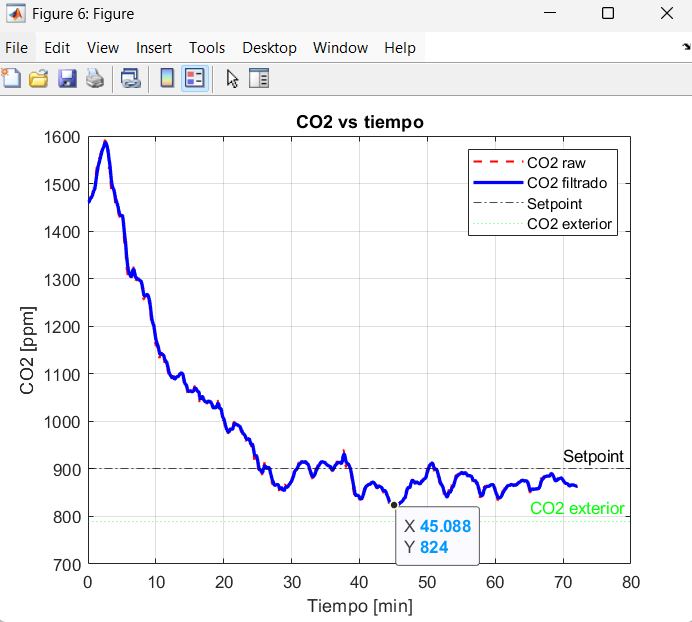
\includegraphics[width=0.9\linewidth]{images/capitulo4/CO2vsTiempo.png}
    \caption{Evolución de la concentración de CO\(_2\) durante la prueba experimental con controlador PI/PID.}
    \label{fig:pid_co2_tiempo}
\end{figure}

Como se observa en la Figura \ref{fig:pid_co2_tiempo}, la concentración de CO\(_2\) inicia en un valor elevado, cercano a 1500 ppm, y posteriormente disminuye de manera progresiva debido a la acción de los ventiladores. El sistema logra aproximarse al setpoint establecido de 900 ppm y luego se mantiene en una zona cercana o inferior a dicho valor. Este comportamiento evidencia que el controlador PI/PID permite reducir la concentración de CO\(_2\) desde una condición inicial desfavorable hasta un rango más adecuado para el ambiente evaluado.

\begin{figure}[H]
    \centering
    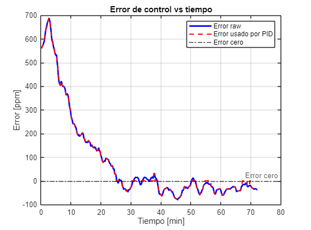
\includegraphics[width=0.9\linewidth]{images/capitulo4/ERRORvsTiempo.png}
    \caption{Evolución del error de control durante la prueba experimental con controlador PI/PID.}
    \label{fig:pid_error_tiempo}
\end{figure}

La Figura \ref{fig:pid_error_tiempo} muestra la evolución del error de control, calculado como la diferencia entre la concentración medida de CO\(_2\) y el setpoint. Al inicio de la prueba, el error es elevado debido a que la concentración de CO\(_2\) se encuentra por encima del valor de referencia. Conforme avanza la ventilación, el error disminuye progresivamente hasta aproximarse a cero. Las oscilaciones posteriores alrededor del error nulo pueden atribuirse al ruido del sensor, a la dinámica propia del ambiente y a las variaciones generadas por la actuación de los ventiladores.

\begin{figure}[H]
    \centering
    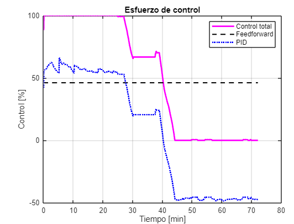
\includegraphics[width=0.9\linewidth]{images/capitulo4/EsfuerzoControl.png}
    \caption{Esfuerzo de control aplicado por el controlador PI/PID.}
    \label{fig:pid_esfuerzo_control}
\end{figure}

En la Figura \ref{fig:pid_esfuerzo_control} se presenta el esfuerzo de control aplicado al sistema. Durante la etapa inicial, la señal de control total se mantiene en valores elevados, debido a que la concentración de CO\(_2\) supera ampliamente el setpoint. A medida que la concentración disminuye, el esfuerzo de control también se reduce, lo cual indica que el controlador disminuye progresivamente la ventilación cuando el sistema se aproxima al valor de referencia.

\begin{figure}[H]
    \centering
    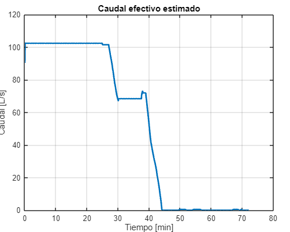
\includegraphics[width=0.9\linewidth]{images/capitulo4/Caudal.png}
    \caption{Caudal efectivo estimado durante la prueba experimental con controlador PI/PID.}
    \label{fig:pid_caudal}
\end{figure}

La Figura \ref{fig:pid_caudal} muestra el caudal efectivo estimado a partir de la señal de control aplicada a los ventiladores. Al inicio de la prueba, el caudal se mantiene en un valor alto debido a la necesidad de reducir rápidamente la concentración de CO\(_2\). Posteriormente, conforme el sistema se acerca al setpoint, el caudal disminuye hasta valores cercanos a cero. Este resultado es coherente con la reducción del esfuerzo de control observada previamente.

\begin{figure}[H]
    \centering
    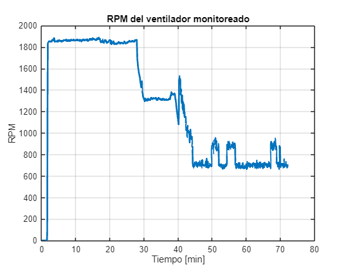
\includegraphics[width=0.9\linewidth]{images/capitulo4/RPM.png}
    \caption{RPM del ventilador monitoreado durante la prueba experimental con controlador PI/PID.}
    \label{fig:pid_rpm}
\end{figure}

Finalmente, la Figura \ref{fig:pid_rpm} presenta la velocidad de giro del ventilador monitoreado. Se observa que, durante los primeros minutos, las RPM se mantienen en valores elevados, lo cual coincide con la alta señal de control aplicada por el controlador. Luego, conforme disminuye el requerimiento de ventilación, las RPM también se reducen. Esta gráfica permite validar que la señal PWM generada por el sistema tiene un efecto directo sobre la actuación física del ventilador.

En conjunto, los resultados experimentales muestran que el controlador PI/PID implementado permite reducir la concentración de CO\(_2\) hasta una zona cercana al setpoint y ajustar progresivamente la ventilación aplicada. Además, las gráficas de esfuerzo de control, caudal y RPM permiten verificar que la disminución de CO\(_2\) está asociada a una actuación real de los ventiladores. No obstante, se observan pequeñas oscilaciones alrededor del valor de referencia, las cuales pueden relacionarse con el ruido de medición, la dinámica del ambiente y la sensibilidad del sistema frente a cambios en la señal PWM.




\section{Página web para la lectura de los sensores}


